\documentclass[12pt]{beamer}
% Add handout to documentclass options if wanted

\usepackage[utf8]{inputenc}
\usepackage[T1]{fontenc}
% \usepackage{babel,textcomp}

\setlength{\arrayrulewidth}{1.6pt}
\renewcommand{\arraystretch}{1.2}
\newlength{\Tcalc}


\usepackage[T1]{fontenc}
\usepackage{graphicx}
\usepackage{amsmath}
\usepackage{amssymb}
\usepackage{amsbsy}
\usepackage{amsfonts}
\usepackage{color}
\usepackage{xcolor}
\usepackage{epstopdf}
\usepackage{fancyvrb}
\usepackage{parskip}
\usepackage{url}
\usepackage{listings}
\usepackage{pifont}% http://ctan.org/pkg/pifont
\newcommand{\cmark}{\ding{51}}%
\newcommand{\xmark}{\ding{55}}%
% \usepackage{tikz}
% \def\checkmark{\tikz\fill[scale=0.4](0,.35) -- (.25,0) -- (1,.7) -- (.25,.15) -- cycle;} 

\definecolor{javared}{rgb}{0.6,0,0} % for strings
\definecolor{javagreen}{rgb}{0.25,0.5,0.35} % comments
\definecolor{javapurple}{rgb}{0.5,0,0.35} % keywords
\definecolor{javadocblue}{rgb}{0.25,0.35,0.75} % javadoc

\lstset{language=Matlab,
basicstyle=\ttfamily
keywordstyle=\color{javapurple},%\bfseries,
stringstyle=\color{javared},
commentstyle=\color{javagreen},
morecomment=[s][\color{javadocblue}]{/**}{*/},
morekeywords={super, with},
% numbers=left,
% numberstyle=\tiny\color{black},
stepnumber=2,
numbersep=10pt,
tabsize=2,
showspaces=false,
% captionpos=b,
showstringspaces=false,
frame=  false,
breaklines=true}

\setbeamertemplate{frametitle}
{\begin{centering}\smallskip
\insertframetitle\par
\smallskip\end{centering}}
\setbeamertemplate{itemize item}{$\bullet$}
\setbeamertemplate{navigation symbols}{}
\setbeamertemplate{footline}[text line]{%
\hfill\strut{%
\scriptsize\sf\color{black!60}%
\quad\insertframenumber
   }%
    \hfill
}

% Define some colors:
\definecolor{DarkFern}{HTML}{407428}
\definecolor{DarkCharcoal}{HTML}{4D4944}
\colorlet{Fern}{DarkFern!85!white}
\colorlet{Charcoal}{DarkCharcoal!85!white}
\colorlet{LightCharcoal}{Charcoal!50!white}
\colorlet{AlertColor}{orange!80!black}
\colorlet{DarkRed}{red!70!black}
\colorlet{LightBlue}{blue!70!white}
\colorlet{DarkBlue}{blue!70!black}
\colorlet{DarkGreen}{green!70!black}

% Use the colors:
\setbeamercolor{title}{fg=Fern}
\setbeamercolor{frametitle}{fg=Fern}
\setbeamercolor{normal text}{fg=DarkCharcoal}
\setbeamercolor{block title}{fg=black,bg=Fern!25!white}
\setbeamercolor{block body}{fg=black,bg=Fern!25!white}
\setbeamercolor{alerted text}{fg=AlertColor}
\setbeamercolor{itemize item}{fg=Charcoal}

\newcommand{\frn}[1]{\textcolor{Fern}{#1}}
\newcommand{\alrt}{\color{AlertColor}}
\newcommand{\drk}{\color{DarkCharcoal}}
\newcommand{\bt}[1]{\textbf{#1}}
\newcommand{\kommando}[1]{\textcolor{AlertColor}{\texttt{\textbackslash #1}}}
\newcommand{\ds}{\displaystyle}


\newcommand{\dd}[1]{\ \text{d}#1}
\newcommand{\f}[2]{\frac{#1}{#2}} 
\newcommand{\beq}{\begin{equation}}
\newcommand{\eeq}{\end{equation}}
\newcommand{\bra}[1]{\langle #1|}
\newcommand{\ket}[1]{|#1 \rangle}
\newcommand{\braket}[2]{\langle #1 | #2 \rangle}
\newcommand{\brakket}[2]{\langle #1 || #2 \rangle}
\newcommand{\braup}[1]{\langle #1 \left|\uparrow\rangle\right.}
\newcommand{\bradown}[1]{\langle #1 \left|\downarrow\rangle\right.}
\newcommand{\av}[1]{\left| #1 \right|}
\newcommand{\op}[1]{\hat{#1}}
\newcommand{\braopket}[3]{\langle #1 | {#2} | #3 \rangle}
\newcommand{\ketbra}[2]{\ket{#1}\bra{#2}}
\newcommand{\pp}[1]{\frac{\partial}{\partial #1}}
\newcommand{\ppn}[1]{\frac{\partial^2}{\partial #1^2}}
\newcommand{\up}{\left|\uparrow\rangle\right.}
\newcommand{\upup}{\left|\uparrow\uparrow\rangle\right.}
\newcommand{\down}{\left|\downarrow\rangle\right.}
\newcommand{\downdown}{\left|\downarrow\downarrow\rangle\right.}
\newcommand{\updown}{\left|\uparrow\downarrow\rangle\right.}
\newcommand{\downup}{\left|\downarrow\uparrow\rangle\right.}
\newcommand{\bupup}{\left.\langle\uparrow\uparrow\right|}
\newcommand{\bdowndown}{\left.\langle\downarrow\downarrow\right|}
\newcommand{\bupdown}{\left.\langle\uparrow\downarrow\right|}
\newcommand{\bdownup}{\left.\langle\downarrow\uparrow\right|}
\renewcommand{\d}{{\rm d}}
\newcommand{\Res}[2]{{\rm Res}(#1;#2)}
\newcommand{\To}{\quad\Rightarrow\quad}
\newcommand{\eps}{\epsilon}
\newcommand{\inner}[2]{\langle #1 , #2 \rangle}
\renewcommand{\u}{\uparrow}
\renewcommand{\d}{\downarrow}
\newcommand{\dddd}{\d\d\d\d}
\newcommand{\uddd}{\u\d\d\d}
\newcommand{\dudd}{\d\u\d\d}
\newcommand{\ddud}{\d\d\u\d}
\newcommand{\dddu}{\d\d\d\u}
\newcommand{\uudd}{\u\u\d\d}
\newcommand{\udud}{\u\d\u\d}
\newcommand{\uddu}{\u\d\d\u}
\newcommand{\duud}{\d\u\u\d}
\newcommand{\dudu}{\d\u\d\u}
\newcommand{\dduu}{\d\d\u\u}
\newcommand{\uuud}{\u\u\u\d}
\newcommand{\uudu}{\u\u\d\u}
\newcommand{\uduu}{\u\d\u\u}
\newcommand{\duuu}{\d\u\u\u}
\newcommand{\uuuu}{\u\u\u\u}
\newcommand{\m}{\text{-}}
\newcommand{\ui}{{\u_1}}
\newcommand{\uii}{{\u_2}}
\newcommand{\uiii}{{\u_3}}
\newcommand{\di}{{\d_1}}
\newcommand{\dii}{{\d_2}}
\newcommand{\diii}{{\d_3}}

\title{Quantum mechanics for \\ many-particle systems}
\author{Jonas van den Brink \\ \url{j.v.brink@fys.uio.no}}
\date{18. december 2014}

\setbeamertemplate{frametitle}{\vspace{0.5cm} \insertframetitle} 

\begin{document}
\pagestyle{empty}

\begin{frame}
\maketitle 
\end{frame}

\begin{frame}[fragile]
\begin{center}
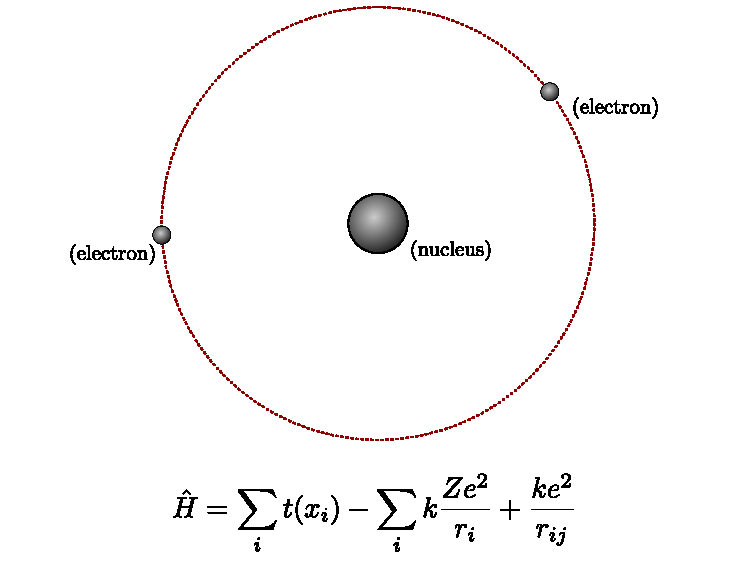
\includegraphics[width=\textwidth]{pres2}
\end{center}
\end{frame}

\begin{frame}[fragile]
Under the {\alrt independant particles} assumption
$$\Psi(x_1, x_2) = \psi_1(x_1) \psi_2(x_2).$$

\visible<2->{
For fermions, we have the anti-symmetric wave function
	$$\Psi(x_1, x_2) = \frac{1}{\sqrt{2}}\big(\psi_1(x_1)  \psi_2(x_2) - \psi_1(x_2)\psi_2(x_1)\big).$$
}

\visible<3->{
For a $N$-particle system, we have the Slater determinant
\begin{align*}
\Psi = \frac{1}{\sqrt{N!}}\det\begin{pmatrix}
\psi_1(r_1) & \psi_1(r_2) &  \ldots & \psi_1(r_N)  \\ 
\psi_2(r_1) & \psi_2(r_2) & \ldots  & \psi_2(r_N)  \\ 
\vdots & \vdots & \ddots & \vdots \\
\psi_N(r_1) & \psi_N(r_2) & \ldots  & \psi_N(r_N)  
\end{pmatrix} = \sqrt{N!}\mathcal{A} \phi_H.
\end{align*}
}
\end{frame}

\begin{frame}[fragile]
{\large \color{DarkFern} We introduce Slater determinants to describe systems of fermions}
\begin{align*}
\Psi = \frac{1}{\sqrt{N!}}\det\begin{pmatrix}
\psi_1(r_1) & \psi_1(r_2) &  \ldots & \psi_1(r_N)  \\ 
\psi_2(r_1) & \psi_2(r_2) & \ldots  & \psi_2(r_N)  \\ 
\vdots & \vdots & \ddots & \vdots \\
\psi_N(r_1) & \psi_N(r_2) & \ldots  & \psi_N(r_N)  
\end{pmatrix}
\end{align*}

\vspace{0.2cm}

Or more compact
$$\Psi = \sqrt{N!}\mathcal{A} \phi_H.$$
\end{frame}



\begin{frame}[fragile]
\begin{center}
{\Huge \color{DarkFern} The Hartree--Fock Method}
\end{center}
\end{frame}

\begin{frame}[fragile]
{\large \color{DarkFern} Variational Principle}
\begin{align*}
\alrt \braopket{\Psi}{\op{H}}{\Psi} & \alrt \geq E_0.
\end{align*}
A method is called \emph{variational} if we can be sure the approximate solutions never undershoot the true ground state.

\begin{align*}
\braopket{\Psi}{\op{H}}{\Psi} &= \sum_{i j}\braket{\Psi}{\phi_i}\braopket{\phi_i}{\op{H}}{\phi_j}\braket{\phi_j}{\Psi} \\
&= \sum_i |C_i|^2 E_i \geq \sum_i |C_i|^2 E_0 \\
&\geq E_0
\end{align*}
\end{frame}

\begin{frame}[fragile]
% {\large \color{DarkFern} Mathematical derivation of the Hartree--Fock method}
Define the energy of a general SD as a functional
$$E[\Phi] = \sum_{p=1}^N \braopket{p}{\op{h}_0}{p} + \frac{1}{2}\sum_{p=1}^N\sum_{q=1}^N\braket{pq|}{pq}.$$

\visible<2->{
Expand the single-particle states into a new (general) basis
\begin{align*}
\sum_{p=1}^N \sum_{\alpha \beta} C^*_{p \alpha} C_{p \beta}\braopket{\alpha}{\op{h}_0}{\beta} + \frac{1}{2}\sum_{pq}^N\sum_{\alpha\beta\gamma\delta} C_{p\alpha}^* C_{q \beta}^* C_{p \gamma} C_{q \delta} \braket{\alpha\beta|}{\gamma\delta}.
\end{align*}}
\end{frame}

\begin{frame}[fragile]
% {\large \color{DarkFern} Mathematical derivation of the Hartree--Fock method}
Minimize $E[\Phi]$ with respect $C_{p\alpha}$, constraint to 
$$\sum_\alpha C_{a \alpha}^* C_{a \alpha} - \delta_{a\alpha} = 0 \quad \forall \quad a.$$

\visible<2->{
Can now use the method of Lagrange multipliers
$$E = E - \sum_a \eps_a \bigg(\sum_\alpha C_{a \alpha}^* C_{a \alpha} - \delta_{a\alpha}\bigg).$$
}

\visible<3->{
To find the minimum, we look for a stationary point
$$\delta E = 0.$$
}
\end{frame}

\begin{frame}[fragile]
{\large \color{DarkFern} The minimization results in the Hartree--Fock equations}

\begin{displaymath}
\color{normal text.fg!0!normal text.bg}
\only<2->{\color{normal text.fg}}
{\usebeamercolor[fg]{text} \sum_\gamma} \underbrace{\usebeamercolor[fg]{text}\bigg(\braopket{\alpha}{\op{h}_0}{\gamma} + \sum_{p=1}^N\sum_{\beta\delta} C_{p\beta}^* C_{p \delta} \braket{\alpha\beta|}{\gamma\delta}\bigg)}_{h_{\alpha\gamma}^{\rm HF}} { \usebeamercolor[fg]{text} C_{k \gamma} = \eps_k C_{k\alpha} \ \forall \ k, \alpha.}
\end{displaymath}

\visible<3->{
$$h^{\rm HF} C_k = \eps_k C_k,$$}
\end{frame}

\begin{frame}[fragile]
{\large \color{DarkFern} The Hartree--Fock method is exactly equivalent to the self-consistent field method}
\begin{center}
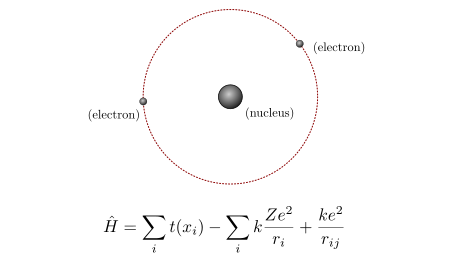
\includegraphics[width=\textwidth]{pres3}
\end{center}
\end{frame}

\begin{frame}[fragile]
{\large \color{DarkFern} The Hartree--Fock method is exactly equivalent to the self-consistent field method}
\begin{center}
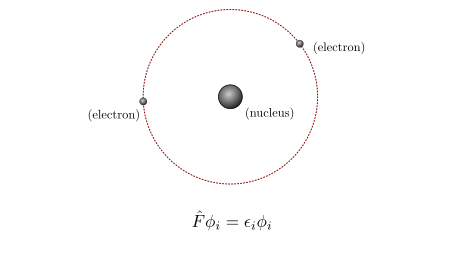
\includegraphics[width=\textwidth]{pres4}
\end{center}
\end{frame}

\begin{frame}[fragile]
\begin{center}
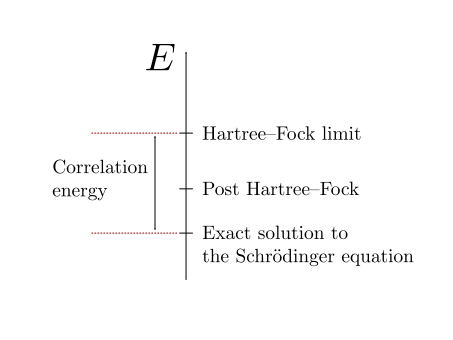
\includegraphics[width=\textwidth]{pres1}
\end{center}
\end{frame}

\begin{frame}[fragile]
\begin{center}
{\Huge \color{DarkFern} Configuration Interaction}
\end{center}
\end{frame}

\begin{frame}[fragile]
{\Huge \color{DarkFern} }
$$\Psi = \Phi_{\rm HF} + \chi_{\rm corr}$$

\visible<2->{
$$\Psi = \Phi_{\rm HF} + \sum_{ai}C_i^{a}\Phi_i^a + \sum_{abij}C_{ij}^{ab}\Phi_{ij}^{ab} + \ldots $$
}

\visible<3->{
The set $\{\Phi_i\}_{i=0}^N$ is an orthonormal basis
}

\visible<4->{
$$H_{ij} = \braopket{\Phi_i}{\op{H}}{\Phi_j}.$$

$$HC = EC.$$
}
\end{frame}

\begin{frame}[fragile]
In {\alrt Full Configuration Interaction} the basis is complete, and the result will be exact.

\vspace{1cm}

\visible<2->{
In practice, one must truncate the configuration space. Usually, including double-excitations is good enough ({\alrt CISD}).
}

\vspace{1cm}

\visible<3->{
The computational cost of CI grows exponentially with the size of the system. It is also not {\alrt extensive}, meaning the energy of a calculation scales erroneously with the system size.	
}
\end{frame}




\begin{frame}[fragile]
\begin{center}
{\Huge \color{DarkFern} Many-Body Perturbation Theory}
\end{center}
\end{frame}

\begin{frame}[fragile]
We now decompose the Hamiltonian
$$\op{H} = \op{H}_0 + \op{V}, \qquad \op{H_0}\Phi_0 = E_0 \Phi_0.$$

\visible<2->{
Remaining part of the Hamiltonian is seen as a perturbation
$$\op{H} = \op{H}_0 + \lambda \op{V}.$$
}

\visible<3->{
We expand the solution as a power series
$$\Psi = \Phi_0 + \chi = \Phi_0 + \lambda\Psi^{(1)} + \lambda^2\Psi^{(2)} + \lambda^3\Psi^{(3)} + \ldots.$$
$$E = E_0 + \Delta E = E_0 + \lambda E^{(1)} + \lambda^2 E^{(2)} + \lambda^3 E^{(3)} + \ldots.$$
}
\end{frame}

\begin{frame}[fragile]
Insert the power series into the Schrödinger equation
$$(\op{H}-E)\Psi = 0.$$
$$(\op{H_0} + \lambda\op{V} - E_{0} - \lambda E^{(1)} -\ldots\big)\big(\Phi_0 + \lambda\Psi^{(1)} + \ldots\big). $$

We can now comparte terms order by order
\begin{align*}
\mbox{(zeroth order) } (\op{H_0} - E_0)\Psi^{(0)} &= 0 \\
\mbox{(first order)  } (\op{H_0} - E_0)\Psi^{(1)} &= (E^{(1)} - \op{V})\Psi^{(0)} \\
\mbox{(second order) } (\op{H_0} - E_0)\Psi^{(2)} &= (E^{(1)} - \op{V})\Psi^{(1)} + E^{(2)}\Psi^{(0)} \\
&\ \, \vdots
\end{align*}
\end{frame}

\begin{frame}[fragile]
{\large \color{DarkFern} We now turn to Rayleigh-Schrödinger perturbation theory}
\begin{align*}
\Psi &= \sum_{m=0}^\infty \bigg[\op{R_0}(\op{V} - \Delta E)\bigg]^m \Phi_0, \\
\Delta E &= \sum_{m=0}^\infty \braopket{\Phi_0}{\op{V}\bigg[\op{R_0}(\op{V} - \Delta E)\bigg]^m}{\Phi_0}.
\end{align*}

\visible<2-> {
\begin{align*}
E^{(1)} &= \braopket{\Phi}{\op{V}}{\Phi}, \\
E^{(2)} &= \braopket{\Phi}{\op{V}\op{R}_0\op{V}}{\Phi}, \\
E^{(3)} &= \braopket{\Phi}{\op{V}\op{R}_0(\op{V}-E^{(1)})\op{R}_0\op{V}}{\Phi}, \\
E^{(4)} &= \braopket{\Phi}{\op{V}\op{R}_0(\op{V}-E^{(1)})\op{R}_0(\op{V}-E^{(1)})\op{R}_0\op{V}}{\Phi} - E^{(2)}\braopket{\Phi}{\op{V}\op{R}_0^2 \op{V}}{\Phi}
\end{align*}	
}
\end{frame}

\begin{frame}[fragile]
\begin{align*}
E^{(1)} &= \braopket{\Phi}{\op{V}}{\Phi}, \\
E^{(2)} &= \braopket{\Phi}{\op{V}\op{R}_0\op{V}}{\Phi}, \\
E^{(3)} &= \braopket{\Phi}{\op{V}\op{R}_0\op{W}\op{R}_0\op{V}}{\Phi}, \\
E^{(4)} &= \braopket{\Phi}{\op{V}\op{R}_0\op{W}\op{R}_0\op{W}\op{R}_0\op{V}}{\Phi} - E^{(2)}\braopket{\Phi}{\op{V}\op{R}_0^2 \op{V}}{\Phi}
\end{align*}

\begin{align*}
\Psi^{(1)} &= \op{R}_0\op{V}\ket{\Phi}, \\
\Psi^{(2)} &= \op{R}_0\op{W}\op{R}_0\op{V}\ket{\Phi}, \\
\Psi^{(3)} &= \op{R}_0\op{W}\op{R}_0\op{W}\op{R}_0\op{V}\ket{\Phi}_0 - \braopket{\Phi}{\op{V}\op{R}_0\op{V}}{\Phi}\op{R}_0^2\op{V}\ket{\Phi}, \\
\end{align*}	
\end{frame}

\begin{frame}[fragile]
{\large \color{DarkFern} Diagrams are often very useful in finding the different contributions
}

First order: $E^{(1)} = \braopket{\Phi}{\op{V}}{\Phi}$
\begin{center}
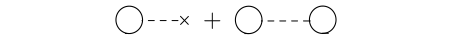
\includegraphics[width=\textwidth]{pres5}	
\end{center}
\visible<2->{$E^{(1)} = \sum_i \braopket{i}{\op{h}_0}{i} + \frac{1}{2}\sum_{ij}\brakket{ij}{ij}$}

\vspace{0.2cm}

\visible<3->{
\hrule
\vspace{0.2cm}

Second order: $E^{(2)} = \braopket{\Phi}{\op{V}\op{R}_0\op{V}}{\Phi}$
\begin{center}

\includegraphics[width=\textwidth]{pres6}	
\end{center}
}
\visible<4->{
$$
E^{(2)} = \displaystyle \frac{1}{4}\sum_{abij}\frac{\brakket{ab}{ij}\brakket{ij}{ab}}{\eps_{ij}^{ab}} + \sum_{ai}\frac{\braopket{a}{\op{f}}{i}\braopket{i}{\op{f}}{a}}{\eps_{i}^a}.
$$
}
\end{frame}

\begin{frame}[fragile]
Third order: $E^{(3)} = \braopket{\Phi}{\op{V}\op{R}_0\op{W}\op{R}_0\op{V}}{\Phi}$
\begin{center}
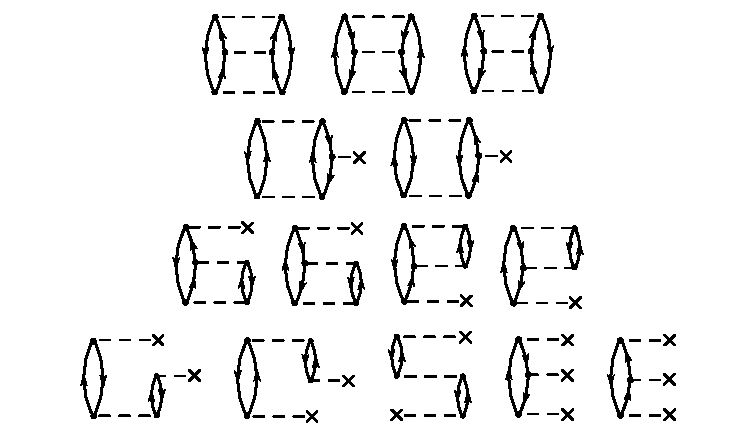
\includegraphics[width=\textwidth]{pres7}	
\end{center}
\end{frame}

\begin{frame}[fragile]
\begin{center}
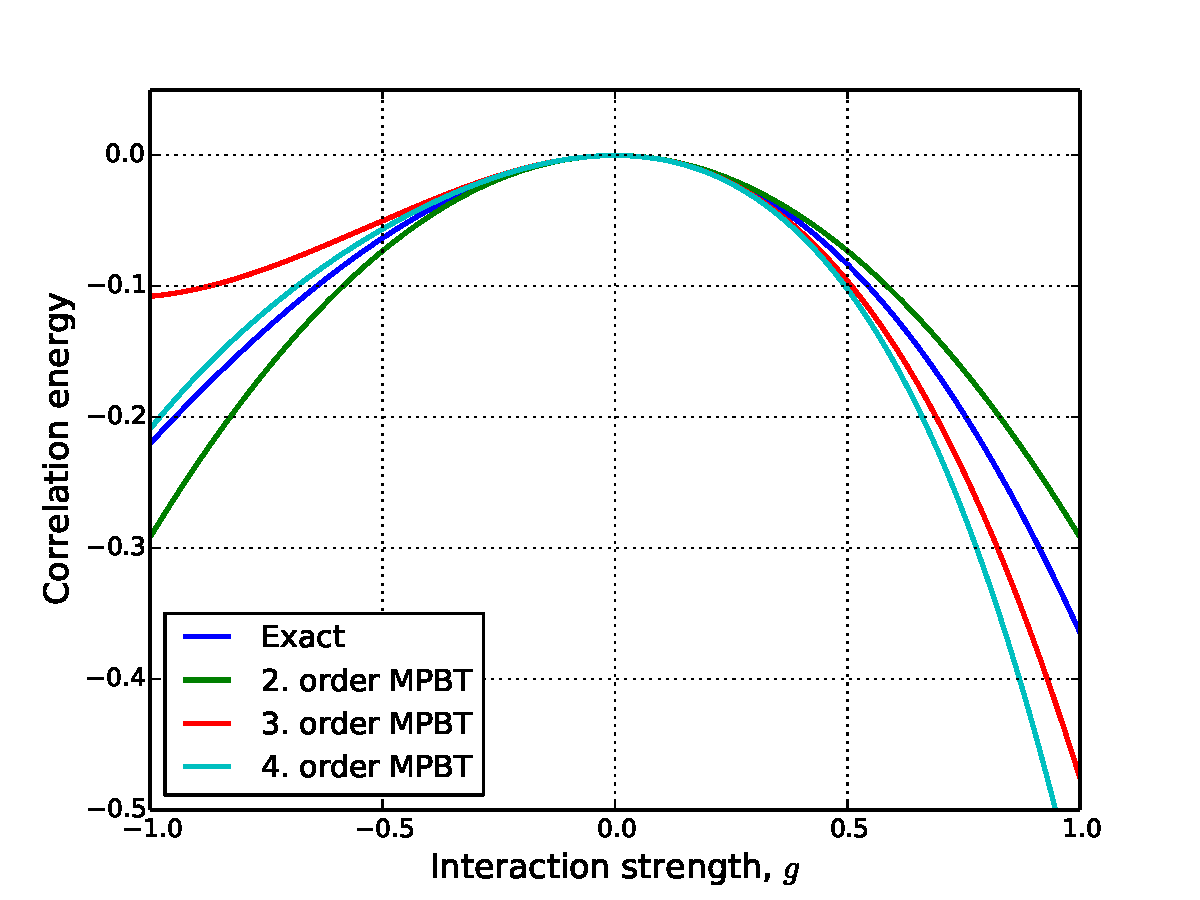
\includegraphics[width=\textwidth]{pert_2}	
\end{center}
\end{frame}

\begin{frame}[fragile]
{\large \color{DarkFern} Goldstones linked diagram theorem}
\begin{center}
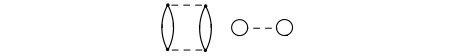
\includegraphics[width=\textwidth]{pres8}	
\end{center}
\end{frame}

\begin{frame}[fragile]
\begin{center}
{\Huge \color{DarkFern} Coupled Cluster}
\end{center}
\end{frame}

\begin{frame}[fragile]
{\large \color{DarkFern} Coupled Cluster is based on the exponential ansatz}
$$\Psi = e^{\op{T}}\Phi_0.$$
\visible<2->{
$$e^{\op{T}} = 1 + \op{T} + \frac{1}{2}\op{T}^2 + \frac{1}{3!}\op{T}^3 + \ldots$$
}

\visible<3->{
The cluster operator is defined as
$$\op{T} = \op{T}_1 + \op{T}_2 + \op{T}_3 + \ldots + \op{T}_N.$$
\begin{align*}
\op{T}_1 &= \sum_{ai} t_i^a \{\op{a}^\dagger \op{i}\} \\
\op{T}_2 &= \sum_{abij} t_{ij}^{ab} \{\op{a}^\dagger \op{i} \op{b}^\dagger \op{j}\}
\end{align*}
}
\end{frame}

\begin{frame}[fragile]
{\large \color{DarkFern} We limit the infinite series by truncating the cluster operator}
$$\op{T}_{\rm CCD} = \op{T}_2, \qquad \op{T}_{\rm CCSD} = \op{T}_1 + \op{T}_2.$$
\visible<2->{
$$\Psi_{\rm CCD} = e^ {\op{T}_2} \Phi_0 = \Phi_0 + \op{T}_2\Phi_0 + \frac{1}{2}\op{T}_2^2\Phi_0 + \frac{1}{3!}\op{T}_2^3\Phi_0+\ldots$$
}

\visible<3->{
The normal-product Schroödinger equation
$$(\op{H}_{\rm N} - \Delta E)e^{\op T}\Phi_{0} = 0.$$
}
\visible<4->{
\begin{displaymath}
\color{normal text.fg!0!normal text.bg}
\only<5->{\color{normal text.fg}}
{\usebeamercolor[fg]{text} (}\underbrace{\usebeamercolor[fg]{text}e^{-\op T}\op{H}_{\rm N}e^{\op T}}_{\mathcal{H}} { \usebeamercolor[fg]{text} - \Delta E)\Phi_{0} = 0}
\end{displaymath}
}
\end{frame}


\begin{frame}[fragile]
{\large \color{DarkFern} We can now find equations for the amplitudes and the correlation energy}
$$(\mathcal{H} - \Delta E)\Phi_0 = 0.$$

\begin{align*}
\braopket{\Phi_0}{\mathcal{H}}{\Phi_0} &= \Delta E, \quad \mbox{(energy equation)} \\
\braopket{\Phi_{ij\ldots}^{ab\ldots}}{\mathcal{H}}{\Phi_0} &= 0. \qquad \, \mbox{(amplitude equation)}
\end{align*}

\visible<2->{
	\hrule
Using Campbell-Baker-Hausdorff expansion, we rewrite
\begin{align*}
\mathcal{H} &= \op{H}_{\rm N} + [\op{H}_{\rm N},\op{T}] + \frac{1}{2!}\big[[\op{H}_{\rm N}, \op{T}], \op{T}\big] + \frac{1}{3!}\bigg[\big[[\op{H}_{\rm N}, \op{T}], \op{T}\big], \op{T}\bigg] + \ldots \\
\visible<3->{&= \big(\op{H}_{\rm N} e^{\op{T}}\big)_{\rm C}}
\end{align*}
}
\end{frame}

\begin{frame}
{\large \color{DarkFern} These are the CC equations}
\begin{align*}
\braopket{\Phi_0}{\op{H}_{\rm N}e^{\op{T}}}{\Phi_0}_{\rm C} &= \Delta E, \quad \mbox{(energy equation)} \\
\braopket{\Phi_{ij\ldots}^{ab\ldots}}{\op{H}_{\rm N}e^{\op{T}}}{\Phi_0}_{\rm C} &= 0. \qquad \, \mbox{(amplitude equation)} 
\end{align*}	
\end{frame}

\begin{frame}
{\large \color{DarkFern} Example: Equation for the energy for CCSD}

$$\op{T} = \op{T}_1 + \op{T}_2 $$
$$\braopket{\Phi_0}{\op{H}_{\rm N}\big(1 + \op{T}_1 + \op{T}_2 + \frac{1}{2}\op{T}_1^2 + \op{T}_1\op{T}_2 + \frac{1}{2}\op{T}_2^2 + \ldots \big)}{\Phi_0}_{\rm C} = \Delta E$$

\visible<2-> {
$$\braopket{\Phi_0}{\op{H}_{\rm N}\big(\op{T}_1 + \op{T}_2 + \frac{1}{2}\op{T}_1^2\big)}{\Phi_0}_{\rm C} = \Delta E$$	
}

\visible<3-> {
\begin{center}

\includegraphics[width=\textwidth]{pres9}	
\end{center}
$$\Delta E = \sum_{ai}f_{ai}t_{i}^a + \frac{1}{2}\sum_{abij}\brakket{ab}{ij}t_{i}^a t_j^b + \frac{1}{4}\sum_{abij}\brakket{ab}{ij}t_{ij}^{ab}.$$
}
\end{frame}





\begin{frame}[fragile]
The \text{\alrt Hartree--Fock method} finds the lowest-energy single SD for the system. It can be found either from a mathematical minimization problem, or from a self-consistent field approach.

A single SD is often to simple, and so HF does not account for the \textbf{electron correlation energy}. Is therefore a good starting point, but rarely sufficient.

The method is both \textbf{variational} and \textbf{extensive}.
\end{frame}

\begin{frame}[fragile]
\text{\alrt Configuration interaction} is the simplest post Hartree-Fock method, both conceptually and computationally---it does however scale poorly with the system size.

FCI always gives the exact result, but is rarely possible.

Truncated CI is \textbf{variational}, but \textbf{not extensive}.
\end{frame}

\begin{frame}[fragile]
\text{\alrt Many-body perturbation theory} results from splitting the Hamiltonian and taking the power-expansion of the perturbed wave-function and energy. We the corrections order-by-order.

It is \textbf{extensive} in every order, but \textbf{not variational}. There is also no guaranteee of convergence.
\end{frame}

\begin{frame}[fragile]
\text{\alrt Coupled cluster} is based on the exponential ansatz. It can be seen as taking certain contributions from MBPT and summing them to infinite order (Shavitt and Bartlett). Alternatively as CI with added complexities (Szabo).

It is therefore \textbf{extensive}, but \textbf{not variational}.  

Just as for CI, CC has to be truncated, but for CCD and CCSD we usually have better results than for CID and CISD.
\end{frame}

\begin{frame}[fragile]
\begin{center}
\begin{tabular}{c|c|c}
  & Variational & Extensive \\ \hline
HF & \color{DarkFern} \cmark & \color{DarkFern} \cmark \\
FCI & \color{DarkFern} \cmark & \color{DarkFern} \cmark \\ \hline
CI & \color{DarkFern} \cmark & \alrt \xmark \\
MBPT & \alrt \xmark & \color{DarkFern} \cmark \\
CC & \alrt \xmark & \color{DarkFern} \cmark
\end{tabular}
\end{center}
\end{frame}

\end{document}